\begin{refsection}

\chapter{\textsuperscript{230}Th--U}\label{ch:ThU-R}

\noindent\begin{minipage}[t]{.3\linewidth}
\strut\vspace*{-\baselineskip}\newline
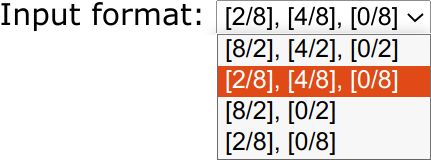
\includegraphics[width=\linewidth]{../figures/ThUformats.png}
\end{minipage}
\begin{minipage}[t]{.7\linewidth}
\texttt{IsoplotR} accepts four types of Th--U data, as
  described in Chapter~\ref{ch:ThU}.
\end{minipage}

\begin{script}
# 238U/232Th, 234U/232Th, 230Th/232Th:
ThU1 <- read.data('ThU1.csv',method='Th-U',format=1)
# 232Th/238U, 234U/238U, 230Th/238U:
ThU2 <- read.data('ThU2.csv',method='Th-U',format=2)
# 238U/232Th, 230Th/232Th:
ThU3 <- read.data('ThU3.csv',method='Th-U',format=3)
# 232Th/238U, 230Th/238U:
ThU4 <- read.data('ThU4.csv',method='Th-U',format=4)
\end{script}

\noindent returns a list with four items:

\begin{enumerate}
\item\texttt{format} stores the value of the eponymous input argument,
\item\texttt{x} is a matrix containing the isotopic ratio measurements.
\item\texttt{Th02} is a two-element vector with the initial
  \textsuperscript{230}Th/\textsuperscript{232}Th activity ratio of
  any detrital component. This information is only relevant to
  formats~1 and 2, and is further discussed below.
\item\texttt{Th02U48} is a nine-element vector with the measured
  composition of the detritus, specified as the
  \textsuperscript{230}Th/\textsuperscript{238}U activity ratio and
  its standard error, the
  \textsuperscript{232}Th/\textsuperscript{238}U activity ratio and
  its standard error, the
  \textsuperscript{234}U/\textsuperscript{238}U activity ratio and its
  standard error, and the respective error correlations of these three
  pairs of activity ratios. Also this information is only relevant to
  formats~1 and 2, as further discussed below.
\end{enumerate}

\noindent\begin{minipage}[t]{.15\linewidth}
\strut\vspace*{-\baselineskip}\newline
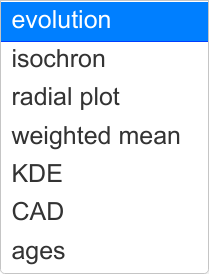
\includegraphics[width=\linewidth]{../figures/ThUplotdevices.png}\\
\end{minipage}
\begin{minipage}[t]{.85\linewidth}
Th--U data can be visualised on six different plot devices.
Additionally, the single aliquot age estimates can also be reported in
a downloadable data table.
\end{minipage}

\noindent\begin{minipage}[t]{.6\linewidth}
\strut\vspace*{-\baselineskip}\newline
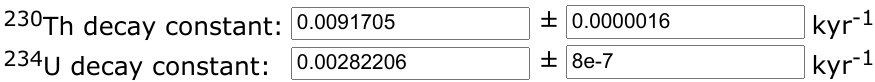
\includegraphics[width=\linewidth]{../figures/ThUlambda.png}
\end{minipage}
\begin{minipage}[t]{.4\linewidth}
  Default values for the decay constants (in kyr$^{-1}$) of
  \textsuperscript{234}U and \textsuperscript{230}Th are taken from
  \citet{cheng2013}.
\end{minipage}

\begin{script}
# query the 234U decay constant:
l34 <- settings('lambda','U234')[1]
# change the 230Th decay constant to match a half-life of 75kyr:
settings('lambda','Th230',log(2)/75)
\end{script}

\section{Isochrons}\label{sec:ThUisochron-R}

\noindent\begin{minipage}[t]{.3\linewidth}
\strut\vspace*{-\baselineskip}\newline
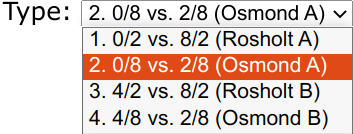
\includegraphics[width=\linewidth]{../figures/ThUisochron12.png}
\end{minipage}
\begin{minipage}[t]{.7\linewidth}
  \texttt{IsoplotR} implements four different types of isochrons for
  Th--U formats~1 and 2, which are based on three-dimensional isotope
  ratio measurements decribing different projections of the
  \textsuperscript{238}U--\textsuperscript{234}U--\textsuperscript{230}Th
  system.
\end{minipage}

\begin{script}
oldpar <- par(mfrow=c(2,2)) # 4 x 4 grid of isochron diagrams
for (i in 1:4){ isochron(ThU1,type=i) }
par(oldpar) # restore the graphics settings
\end{script}

\noindent\begin{minipage}[t]{.3\linewidth}
\strut\vspace*{-\baselineskip}\newline
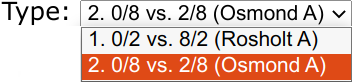
\includegraphics[width=\linewidth]{../figures/ThUisochron34.png}
\end{minipage}
\begin{minipage}[t]{.7\linewidth}
  Th--U formats 3 and 4 assume secular equilibrium between
  \textsuperscript{234}U and \textsuperscript{238}U. Consequently,
  there are only two isochron options for these formats.
\end{minipage}

\begin{console}
isochron(ThU3,type=1) # 230Th/232Th vs. 238U/232Th
\end{console}

Isochron regression for formats 1 and 2 is done using the algorithm of
\citet{ludwig1994}. For formats 3 and 4, the two-dimensional algorithm
of \citet{york2004} is used.\\

\noindent\begin{minipage}[t]{.45\linewidth}
\strut\vspace*{-\baselineskip}\newline
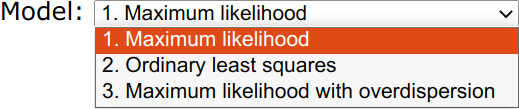
\includegraphics[width=\linewidth]{../figures/PbPbIsochronModels.png}
\end{minipage}
\begin{minipage}[t]{.55\linewidth}
  Any excess dispersion of the data around the best fit line can be
  handled in the usual three ways, which either 1) attribute the
  excess scatter to a multiplicative dispersion term, 2) ignore the
  analytical uncertainties, or 3) attribute the excess scatter to an
  additive dispersion term (Figure~\ref{fig:isochronMSWD}).
\end{minipage}

\begin{script}
# Ludwig and Titterington (1993) regression of 230Th/238U vs. 232Th/238U
isochron(ThU1,type=3,model=1)
\end{script}

\noindent\begin{minipage}[t]{.25\linewidth}
\strut\vspace*{-\baselineskip}\newline
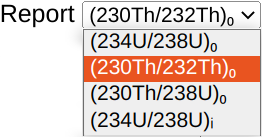
\includegraphics[width=\linewidth]{../figures/ThUy0.png}
\end{minipage}
\begin{minipage}[t]{.75\linewidth}
Along with the isochron age, \texttt{IsoplotR} can also report 1) the
authigenic \textsuperscript{234}U/\textsuperscript{238}U activity
ratio; 2) authigenic \textsuperscript{230}Th/\textsuperscript{232}Th
activity ratio; 3) detrital
\textsuperscript{230}Th/\textsuperscript{238}U activity ratio; or 4)
initial \textsuperscript{234}U/\textsuperscript{238}U activity ratio.
\end{minipage}

\begin{script}
isochron(ThU1,type=3,model=1,y0option=2)
\end{script}

All the other isochron options are as in the generic regression
function of Section~\ref{sec:OtherRegression}.

\section{Evolution diagrams}

Th--U diagrams also work differently for formats~1 and 2 than they do
for formats~3 and 4.

\begin{enumerate}

\item For the
  \textsuperscript{238}U--\textsuperscript{234}U--\textsuperscript{230}Th
  data of formats~1 and 2, the data can either be plotted as
  \textsuperscript{234}U/\textsuperscript{238}U-activity ratios
  against \textsuperscript{230}Th/\textsuperscript{238}U-activity
  ratios:

\begin{console}
evolution(ThU2)
\end{console}

  \noindent\begin{minipage}[t]{.4\linewidth}
  \strut\vspace*{-\baselineskip}\newline
  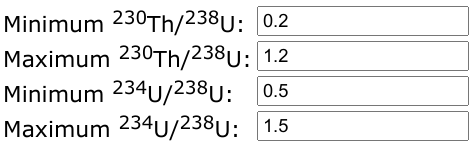
\includegraphics[width=\linewidth]{../figures/ThUformat12evolutionLimits.png}
  \end{minipage}
  \begin{minipage}[t]{.6\linewidth}
    The axis limits of this type of evolution diagram can be specified in
    terms of the \textsuperscript{230}Th/\textsuperscript{238}U and
    \textsuperscript{234}U/\textsuperscript{238}U activity ratios.
  \end{minipage}

\begin{console}
evolution(ThU2,xlim=c(0.2,1.2),ylim=c(0.5,1.5))
\end{console}

  \noindent\begin{minipage}[t]{.3\linewidth}
  \strut\vspace*{-\baselineskip}\newline
  
\includegraphics[width=\linewidth]{../figures/ThUvsAge.png}
  \end{minipage}
  \begin{minipage}[t]{.7\linewidth}
    Alternatively, the same data can also be visualised as initial
    \textsuperscript{234}U/\textsuperscript{238}U-ratios against
    \textsuperscript{230}Th-\textsuperscript{234}U-\textsuperscript{238}U-ages.
  \end{minipage}

\begin{console}
evolution(ThU2,transform=TRUE)
\end{console}

  \noindent\begin{minipage}[t]{.4\linewidth}
  \strut\vspace*{-\baselineskip}\newline
  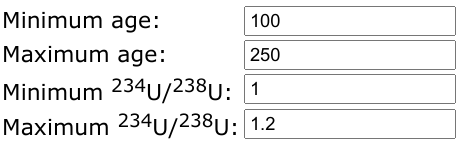
\includegraphics[width=\linewidth]{../figures/ThUvsAgeLimits.png}
  \end{minipage}
  \begin{minipage}[t]{.6\linewidth}
    In this case the axis limits are defined in terms of ages (in ka)
    and \textsuperscript{234}U/\textsuperscript{238}U-activity ratios.
  \end{minipage}

\begin{console}
evolution(ThU2,transform=TRUE,xlim=c(100,250),ylim=c(1,1.2))
\end{console}

  In either case, the detrital \textsuperscript{230}Th component can
  (optionally) be removed in one of three ways:

\begin{enumerate}
  \item \begin{minipage}[t]{.4\linewidth}
    \strut\vspace*{-\baselineskip}\newline
    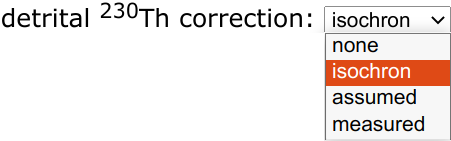
\includegraphics[width=\linewidth]{../figures/ThUdetritalisochroncorr.png}
  \end{minipage}
    \begin{minipage}[t]{.6\linewidth}
      A first option is to use the inferred detrital
      \textsuperscript{230}Th/\textsuperscript{232}Th-ratio obtained
      by three-dimensional (model-1) isochron regression.
    \end{minipage}

\begin{console}
evolution(ThU1,detritus=1)
\end{console}

  \item \begin{minipage}[t]{.7\linewidth}
    \strut\vspace*{-\baselineskip}\newline
    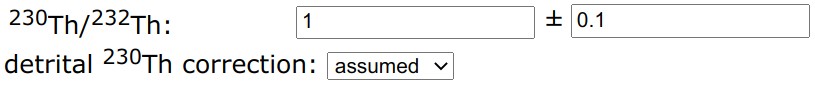
\includegraphics[width=\linewidth]{../figures/ThUinitialThassumed.png}
  \end{minipage}
    \begin{minipage}[t]{.3\linewidth}
      A nominal detrital Th-correction requires the initial
      \textsuperscript{230}Th/\textsuperscript{232}Th-activity ratio
      of the detritus.\\
    \end{minipage}

    At the CLI, the initial
    \textsuperscript{230}Th/\textsuperscript{232}Th-activity ratio
    must be provided to \texttt{IsoplotR} via the \texttt{read.data()}
    function:

\begin{script}
ThU2b <- read.data('ThU2.csv',method='Th-U',format=2,Th02=c(1,0.1))
evolution(ThU2b,detritus=2)
\end{script}

\item Finally, the third way to correct for detrital
  \textsuperscript{230}Th is to measure the present day
  \textsuperscript{230}Th--\textsuperscript{232}Th--\textsuperscript{234}U--\textsuperscript{238}U
  activities of the detritus:\\

  \noindent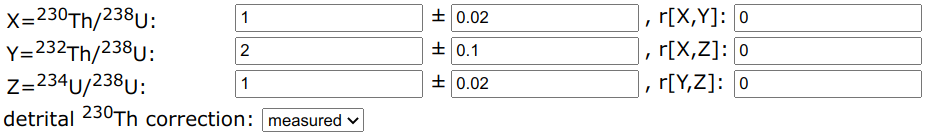
\includegraphics[width=\linewidth]{../figures/ThUmeasureddetritus.png}\\

 Again, the CLI accommodates these measurements via the
 \texttt{read.data()} function:

\begin{script}
ThU2c <- read.data('ThU2.csv',method='Th-U',format=2,
                   Th02U48=c(1,0.02,2,0.1,1,0.1,0,0,0))
evolution(ThU2c,detritus=3)
\end{script}

\noindent where \texttt{Th02U48} contains the measured composition of
the detritus, expressed as a 9-element vector containing the
\textsuperscript{230}Th/\textsuperscript{238}U,
\textsuperscript{232}Th/\textsuperscript{238}U and
\textsuperscript{234}U/\textsuperscript{238}U activity ratios and
their standard errors, as well as the error correlations between them.

\end{enumerate}

\item For Th--U formats~3 and 4, the evolution plot is simply a
  Rosholt type-A annotated with a grid of isochron lines.

\begin{console}
evolution(ThU3)
\end{console}

\item For all four Th--U formats, the isochron fit can be projected
  onto the evolution diagram.\\

  \begin{minipage}[t]{.55\linewidth}
    \strut\vspace*{-\baselineskip}\newline
    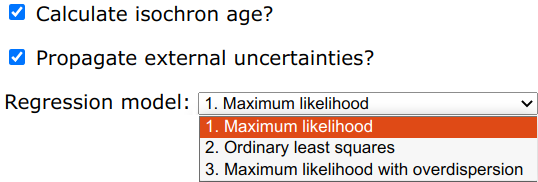
\includegraphics[width=\linewidth]{../figures/ThUevolutionIsochron.png}
  \end{minipage}
  \begin{minipage}[t]{.45\linewidth}
    Ticking the `Calculate isochron age' box adds a pull-down menu
    to the GUI with the same three fit models as for the isochron
    plot of Section~\ref{sec:ThUisochron-R}, as well as a selection
    box to propagate the decay constant uncertainties into the
    isochron age. Unticking the `Calculate isochron age' box hides
    these options.
  \end{minipage}

\begin{console}
evolution(ThU1,isochron=TRUE,model=1,exterr=TRUE)
\end{console}

\item\begin{minipage}[t]{.5\linewidth}
    \strut\vspace*{-\baselineskip}\newline
    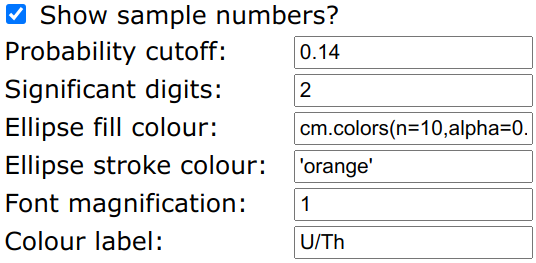
\includegraphics[width=\linewidth]{../figures/ThUevolutionOtherOptions.png}
  \end{minipage}
  \begin{minipage}[t]{.5\linewidth}
    The remaining options of the Th--U evolution function allow the
    user to add sample numbers to the error ellipses, specify the
    significance level of those ellipses (as well as the confidence
    intervals of any isochron output), and assign a bespoke fill and
    stroke colour to them.
  \end{minipage}

  Reporting the isochron uncertainties as relative `2-sigma' errors,
  and colouring the error ellipses by U/Th ratio:

\begin{script}
evolution(ThU1,oerr=5,levels=ThU1$x[,'U238Th232'],clabel='U/Th',
          ellipse.fill=c('#A1B2C380','#FF000080'),
          ellipse.stroke='#1A2B3C00')
\end{script}

\end{enumerate}

\section{Ages}\label{sec:ThU-ages-R}

Although Th--U data are usually measured in multiple cogenic aliquots,
\texttt{IsoplotR} also allows each aliquot to be assigned a separate
age. Like the \texttt{evolution} function, also the \texttt{age}
function behaves in a slightly different way for Th--U formats~1 and
2, and formats 3 and 4, respectively.

\begin{enumerate}

\item For Th--U formats~1 and 2, there are four options to deal with
  the detrital \textsuperscript{230}Th component. The first is to
  ignore it. This is equivalent to assuming a zero initial
  \textsuperscript{230}Th/\textsuperscript{232}Th-activity ratio in
  the detritus.

  \begin{enumerate}
  
  \item \begin{minipage}[t]{.4\linewidth}
    \strut\vspace*{-\baselineskip}\newline
    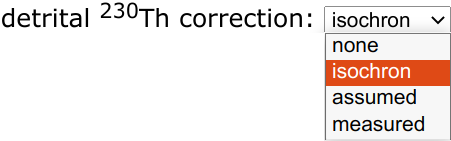
\includegraphics[width=\linewidth]{../figures/ThUdetritalisochroncorr.png}
  \end{minipage}
    \begin{minipage}[t]{.6\linewidth}
      A second option is to use the inferred detrital
      \textsuperscript{230}Th/\textsuperscript{232}Th-ratio obtained
      by three-dimensional (model-1) isochron regression.
    \end{minipage}

\begin{console}
age(ThU1,detritus=1)
\end{console}

\item \begin{minipage}[t]{.7\linewidth}
    \strut\vspace*{-\baselineskip}\newline
    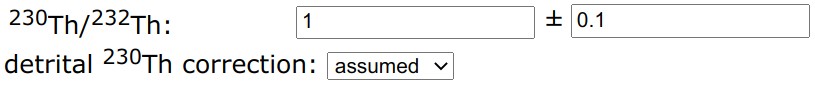
\includegraphics[width=\linewidth]{../figures/ThUinitialThassumed.png}
  \end{minipage}
    \begin{minipage}[t]{.3\linewidth}
      A nominal detrital Th-correction requires the initial
      \textsuperscript{230}Th/\textsuperscript{232}Th-activity ratio
      of the detritus.\\
    \end{minipage}

    At the CLI, the initial
    \textsuperscript{230}Th/\textsuperscript{232}Th-activity ratio
    must be provided to \texttt{IsoplotR} via the \texttt{read.data()}
    function:

\begin{script}
ThU2b <- read.data('ThU2.csv',method='Th-U',format=2,Th02=c(1,0.1))
age(ThU2b,detritus=2)
\end{script}

\item Finally, the third way to correct for detrital
  \textsuperscript{230}Th is to measure the present day
  \textsuperscript{230}Th--\textsuperscript{232}Th--\textsuperscript{234}U--\textsuperscript{238}U
  activities of the detritus:\\

  \noindent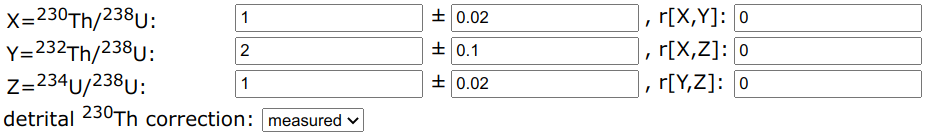
\includegraphics[width=\linewidth]{../figures/ThUmeasureddetritus.png}\\

 Again, the CLI accommodates these measurements via the
 \texttt{read.data()} function:

\begin{script}
ThU2c <- read.data('ThU2.csv',method='Th-U',format=2,
                   Th02U48=c(1,0.02,2,0.1,1,0.1,0,0,0))
age(ThU2c,detritus=3)
\end{script}

\end{enumerate}

\item The detrital \textsuperscript{230}Th-correction does not apply
  to Th--U formats~3 and 4. Instead, the initial
  \textsuperscript{230}Th component can be corrected for in two ways:

  \begin{enumerate}

\item\begin{minipage}[t]{.7\linewidth}
    \strut\vspace*{-\baselineskip}\newline
    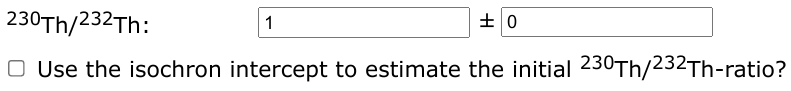
\includegraphics[width=\linewidth]{../figures/ThUformat34initial02.png}
  \end{minipage}
    \begin{minipage}[t]{.3\linewidth}
      A nominal detrital Th-correction requires the initial
      \textsuperscript{230}Th/\textsuperscript{232}Th-activity ratio
      of the rock.\\
    \end{minipage}    

\begin{script}
ThU3b <- read.data('ThU3.csv',method='Th-U',format=3,Th02=c(1,0))
age(ThU3b,i2i=FALSE)
\end{script}

    
\item\begin{minipage}[t]{.7\linewidth}
    \strut\vspace*{-\baselineskip}\newline
    
\includegraphics[width=\linewidth]{../figures/ThUi2i.png}
  \end{minipage}
    \begin{minipage}[t]{.3\linewidth}
      Alternatively, the initial
      \textsuperscript{230}Th/\textsuperscript{232}Th-activity ratio
      can also be inferred by isochron regression.\\
    \end{minipage}    

\begin{console}
age(ThU3,i2i=TRUE)
\end{console}

  \end{enumerate}
  
\end{enumerate}

\section{Radial, weighted mean, KDE and CAD plots}

The \texttt{radial()}, \texttt{weightedmean()}, \texttt{kde()} and
\texttt{cad()} function(s) combine the settings of the \texttt{age()}
function (Section~\ref{sec:ThU-ages-R}) with their generic versions
(Sections~\ref{sec:OtherRadial}--\ref{sec:OtherCAD}). Here are some
CLI examples:

\begin{enumerate}

\item A radial plot of uncorrected carbonate Th--U aliquots that are
  numbered in blue, except for the first aliquot, which is omitted
  from the central age calculation but is shown in the default grey
  colour:
  
\begin{console}
radialplot(ThU1,show.numbers=TRUE,col='blue',detrital=0,omit=1)
\end{console}

\item A ranked weighted mean plot of carbonate Th--U data whose
  detrital \textsuperscript{230}Th component has been corrected based
  on its measured \textsuperscript{230}Th, \textsuperscript{232}Th,
  \textsuperscript{234}U and \textsuperscript{238}U activities:

\begin{console}
weightedmean(ThU2c,detritus=3,ranked=TRUE)
\end{console}

\item A KDE of volcanic Th--U measurements whose initial
  \textsuperscript{230}Th component was estimated by isochron
  regression, plotted on a logarithmic scale from 120 to 200~ka with a
  kernel bandwidth and histogram bin width of 5\%:

\begin{console}
kde(ThU3,i2i=TRUE,log=TRUE,from=120,to=200,bw=0.05,binwidth=0.05)
\end{console}

\item A CAD of volcanic Th--U measurements whose initial
  \textsuperscript{230}Th component was removed using a nominal
  \textsuperscript{230}Th/\textsuperscript{232}Th-activity ratio:

\begin{console}
cad(ThU3b,i2i=FALSE)
\end{console}
  
\end{enumerate}

\printbibliography[heading=subbibliography]

\end{refsection}
